%!TEX root = SYN.tex

\chapter[Approach]{Approach}
\graphicspath{ {images/approach} }

Comprehending the evolution of a software system is a complex activity, mainly because of the sheer amount of data and its complexity. 
The term \quotes{software evolution} was coined for the first time by Lehman in 1985 in a set of laws \cite{Lehman1985}.
He stated that the complexity of a system is destined to increase over time as the system needs to be adapted to its evolutionary environments. 
To be maintained, software systems need to be comprehended by developers, and this activity can be supported with software visualization. 

The development activity is often supported by a Version Control System (VCS) software for tracking and managing file changes. VCSs have been widely adopted for the last 40 years. Revision Control System (RCS) is one of the oldest, and it was introduced in 1980. Consequently, between 1990 and 2020, developers introduced several VCSs. The most important ones were Concurrent Versions System (CVS) introduced in 1990, Perforce (1995), Subversion (2000), Mercurial, and Git (2005).

One of the most adopted ones is Git, introduced in 2005 by Linus Torvalds\footnote{\url{https://github.com/git/git/commit/e83c5163316f89bfbde7d9ab23ca2e25604af290}}. Millions of repositories use it on GitHub and GitLab. 
For this reason, we focused on systems versioned with this protocol.
Git is a versioning control system that tracks all the changes made to every system file. 
Internally git holds all the information we need to reconstruct the history of a repository. 

In this chapter, we present our sensorial approach to visualizing a software system using a visual and auditive depiction of its evolution. 
To fulfill this purpose, we leverage synesthesia, the production of a sense impression relating to one sense by stimulation of another sense.
Moreover, we also present how we reconstruct and model the history of a repository. 

In this chapter, we present the three main steps of our approach as follows:
\begin{itemize}
    \item first, we model the system's evolution; 
    \item next, we visualize it;
    \item finally, complement the visualization with an auditive portrayal of evolutionary data. 
\end{itemize}

\newpage
\section{Evolution Model}
\label{s:EvolutionModel}

\begin{figure}[H]
    \begin{center}
        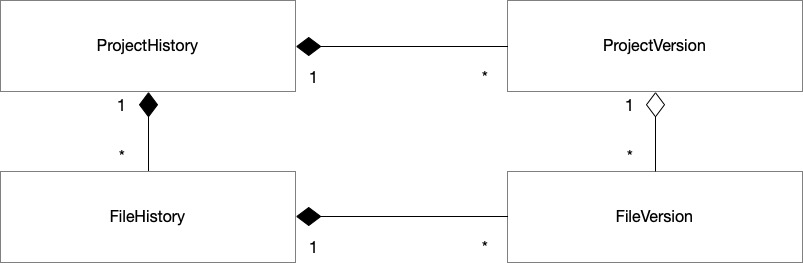
\includegraphics[width=0.6\textwidth]{EvolutionModel.jpg}
    \end{center}
    \caption{Evolutionary Model}
    \label{fig:EvolutionaryModel}
\end{figure}
Various approaches have been proposed to analyze aspects of software evolution. In 2005, Tudor Girba presented Hismo \cite{Girba2005}, a model centered around the notion of history as a first-class entity. Our approach is based on this work. The need to develop a novel evolutionary model comes from the fact that Hismo was designed to work with another versioning system: Subversion (SVN). 
There are several differences between SVN and git. In terms of design, the most important is how they track changes. 
SVN works with the concept of "snapshot" while git works with the concept of "commits". In SVN, when a file has been changed, a new revision of the whole system is created, and consequently, the number of revisions is incremented. 
In contrast, in git, only the modified files would get committed, and thus we don't have a new snapshot of the system every time. 
Therefore, we took Hismo as the starting point of our model and adapted it to the git protocol. 
The Hismo model was based on three concepts:
\begin{itemize}
    \item Snapshot. A representation of the entity whose evolution is studied.
    \item Version. A representation of a system's version. It defines the time when a snapshot was made. 
    \item History. An entity that holds a set of Versions.
\end{itemize}

We replaced the concept of Snapshot with a FileVersion. It represents the version of a file at a particular point in time. Instead of being related to every version of the system, it is related only to the Versions when the file was updated.
Moreover, we made a distinction between File entities and Project entities. So, we mapped the concept of History to FileHistory and the idea of Version to ProjectVersion. 
The entity responsible for holding both of them is called ProjectHistory. \autoref{fig:EvolutionaryModel} depicts the relationships among these concepts. 
To summarize, these are the four main concepts of our evolutionary model: 
\begin{itemize}
    \item \textbf{ProjectHistory}: represents the history of a repository. It holds two sets: a set of FileHistories and a set of ProjectVersions. 
    \item \textbf{FileHistory}: represents a file inside the repository. We consider each file as an entity of the system. Even if the entity's name or location is changed, our model will treat it as the same. So, our approach is resilient to renaming and moving activities. Each FileHistory holds a set of FileVersions, each representing a different version of the entity at a particular point in time.  
    \item \textbf{ProjectVersion}: represents a commit or a version of the system. 
    For each changed file inside a commit, the respective ProjectVersion contains a FileVersion representing that change.
    A ProjectVersion holds contextual information about the commit, such as its timestamp, hash, and message.
    \item \textbf{FileVersion}: represents the version of a file at a particular point in time.
    It is responsible for holding all the evolutionary information of an entity, such as the last action on a file. 
\end{itemize}

\subsection{Historical information retrieval}
To model the history of a repository, we need to extract the historical information from git.
Git works with the concept of branches. Each branch can be seen as a different repository timeline.
Usually, developers use branches to develop features and merge the developed code in a branch that contains the stable codebase.
They create a "merge commit" to do that. 
Each time developers create a new git commit, they deploy a new version of the system that records all the changes made to the commits' tracked files. 
Internally, in git, all git stores all the commits as nodes of a commit-tree. 
The root node represents the repository's first commit and has no parents. 
All the other nodes represent the commits made during the whole lifecycle of the repository. 
Each commit usually has only one parent representing the previous commit.
There is one case where a commit might have more than one parent: merges commits.

Each repository should have a branch containing stable, production-ready code as a convention. Usually, this branch is named "main" or "master". 
In our approach, we aim to analyze the timeline of this stable branch. We start from the root of the commit tree, which represents the initial commit, and then we traverse the whole tree. 
We do not consider "merge commits" during this process since they already incorporate previous commits, and thus they would be considered twice. 
Once we have extracted all the valid commits that reside on the stable branch, we need to extract all the representative information for a ProjectVersion. \\

Git can recognize the following file actions:
\begin{itemize}
    \item \textbf{ADD}. A file is added to the repository.
    \item \textbf{DELETE}. A file has been removed from the repository.
    \item \textbf{MODIFY}. The contents of a file have been modified.
    \item \textbf{RENAME}. A file's name has been changed but the file remained in the same parent directory.
    \item \textbf{MOVE}. A file was moved from one location to another. This action is detected whether the file's name remains the same. 
\end{itemize}

From a commit, we could also extract additional information such as the name of the file being modified, the action made on a file, the number of lines added and removed, and the file paths before and after the changes.
We used the commit's information to track all the paths of an entity. We can update the entity path when it was renamed or moved to follow it during its lifecycle. \\
%\linebreak
When we reconstruct the history of a repository, each FileHistory starts with a FileVersion representing an ADD action.
During the lifecycle of a repository, files can be deleted. In this case, the last FileVersion held by a deleted FileHistory represents a DELETE action.

\begin{figure}
    \begin{center}
        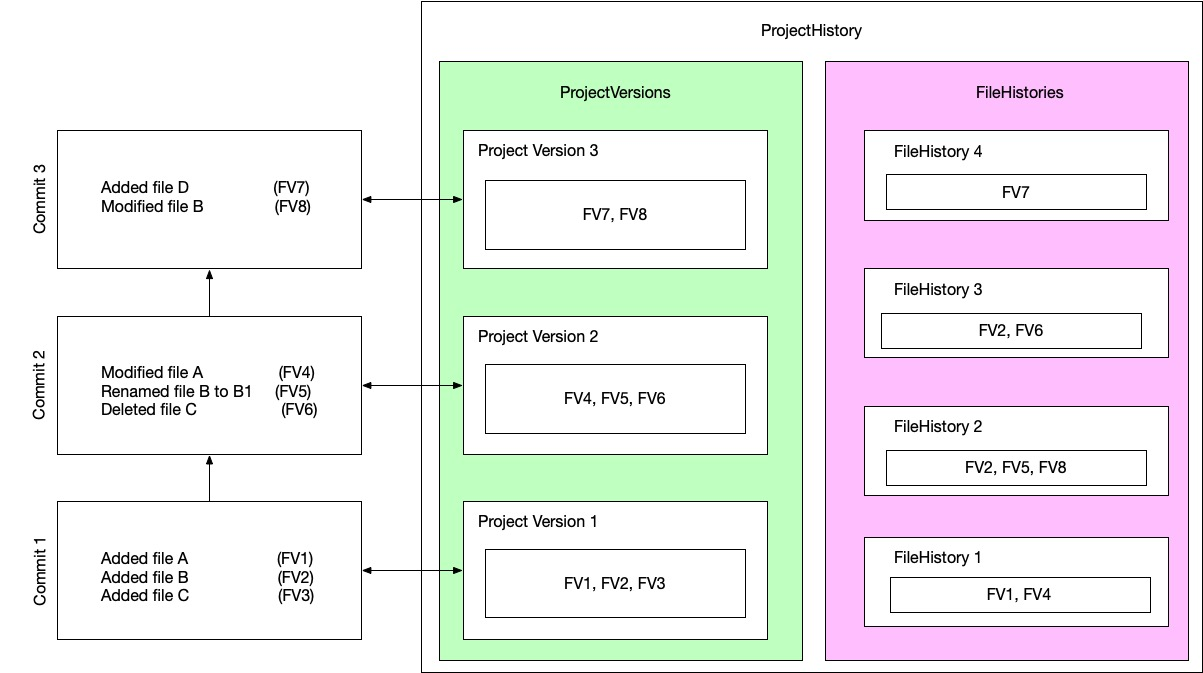
\includegraphics[width=0.8\textwidth]{RebuildingHistory.jpg}
    \end{center}
    \caption{Rebuilding history example}
    \label{fig:RebuildingHistory}
\end{figure}

\autoref{fig:RebuildingHistory} shows an example of building an instance of the evolution model.
First, we create a ProjectHistory with a set of ProjectVersions and a set of FileHistories.
After that, we start to traverse the repository's commit tree.
For each commit, we create a new ProjectVersion that represents a new version of the system. 
We inspect the commit's changelog and create a new FileVersion for each list entry.
Every time we find a newly added file in the changelog of a commit, we create a new FileHistory. 
In the example, in version 1, three new files were added to the repository (A, B, C). Thus, three new FileHistories were created.
Each change was mapped to a FileVersion (FV) and consequently added to the respective FileHistory and ProjectVersion. 
We did the same for ProjectVersions 2 and 3. 

\label{sec:partialHistoricalRepr}
\subsection{Partial historical representation}
\begin{figure}[ht]
    \begin{center}
        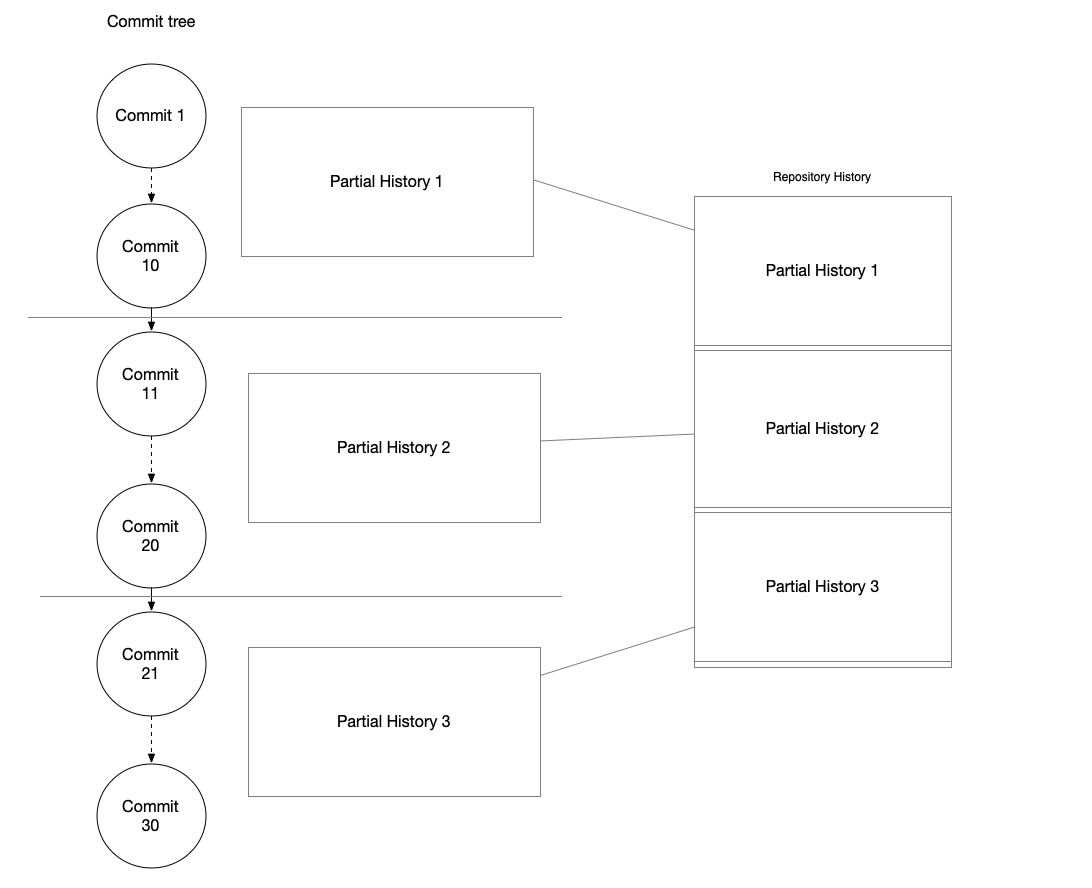
\includegraphics[width=0.5\textwidth]{PartialHistory.png}
    \end{center}
    \caption{Partial history example}
    \label{fig:PartialHistory}
\end{figure}
We had as a goal to develop a scalable approach to mine software repositories. This way, it should always be possible to analyze large repositories in an acceptable amount of time. 
In other words, our approach needs to be scalable.
GitHub host the code of some notorious open-source systems, such as LibreOffice, Elasticsearch, and Linux.
They all have more than 500,000 commits each. Thus, we cannot aim to reconstruct their histories with a single analyzer, as it would take too much time.  
At the time of writing, the repository of Linux had 1,090,563 commits. 
To checkout from one commit to another, we could assume that git needs one second. 
As a result, just to navigate through the whole history of Linux, we would need 11 days.
Moreover, in this simple estimation, we are omitting the time the analyzer needs to extract metrics from every file on each version. 

To overcome this mining issue, we present a scalable approach based on the concept of partial history.
A partial history holds information about a specific range of time of the ProjectHistory. 
It can be seen as a subset of a ProjectHistory. 
We can split the repository's history into multiple parts, each represented by a partial record. Then when all the analyses are completed, we merge them to reconstruct the whole story of the repository.


\autoref{fig:PartialHistory} shows an example PartialHistory representation. 
We split the commit tree into multiple chunks and then run the analysis on each. 
In the end, the final history will be represented by merging all the PartialHistories. 
Nonetheless, we can build PartialHistories in parallel, but we cannot do the same for the final History, 
because the final merge needs to be done sequentially. The sequence needs to follow the order of the commit tree. 
In \autoref{fig:PartialHistory}, for example,
PartialHistory1 represents the history from commit 1 to commit 10, 
PartialHistory2 represents the history from commit 11 to commit 20, and 
PartialHistory3 represents the history from commit 21 to commit 30.
Therefore, the commit order is respected if we merge them in this order: 1, 2, 3. 
The result of a single analysis and a parallel analysis must be identical. 
To ensure that, we need to pay attention to the merge operations of our analysis.
When we merge the history of a repository with a partial history, we need to preserve the characteristics of our model. 
In particular, if FileHistory is already present in our history, we do not have to duplicate it, but instead, we need to update it. 
\label{s:evolutionaryMetrics}
\subsection*{Evolutionary metrics}

\begin{table}[ht]
    \centering
        \begin{tabular}{@{}ll@{}} 
        \toprule
        \textbf{FileType} & \textbf{Metrics} \\\midrule
        File    & SIZE      \\
        Textual & LOC, LinesAdded, LinesRemoved, SIZE \\
        Binary  & SIZE         \\
        Java    & SLOC, LOC, LinesAdded, LinesRemoved, SIZE \\
        JPEG    & SIZE \\\bottomrule
    \end{tabular}
    \caption{Example of metrics collected and inherited for each FileType}
    \label{table:metricsT}
\end{table}

Every version of the system holds a set of files. 
Each file is represented by a FileVersion, which is part of a FileHistory.
For the visualization, we collect metrics representing the files' states.
Since we aim to have a language-agnostic approach, we selected only language-agnostic metrics. 
However, the set of metrics can be easily extended.
We defined a taxonomy to classify and categorize all the files in a system. 
Each category is then mapped to a set of metrics. Metrics can also be inherited from parent categories. 

\autoref{fig:taxonomy} shows an example of a possible taxonomy definition. \autoref{table:metricsT} shows the final set of metrics associated with each file type. We compute the metric SIZE for each file type since it is inherited from the root file type. Moreover, Java FileType also inherits the metrics of the Textual FileType.  

\begin{figure}[ht]
    \centering
    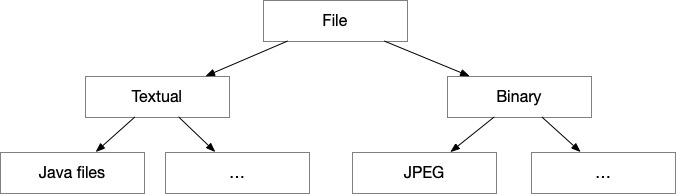
\includegraphics[width=0.5\textwidth]{Taxonomy.jpg}
    \caption{Example of a file type's taxonomy}
    \label{fig:taxonomy}
\end{figure}



We defined a set of metrics as can be seen in \autoref{table:metricsT}. We collect the file's size, the number of Lines of Code (LOC), the number of Source Lines of Code (SLOC) by ignoring comments and empty lines, and the number of lines added and removed. These are basic source code metrics to demonstrate our approach. The list can be extended with additional metrics depending on the purpose.


\section{Visualization}
We represent a ProjectHistory with two kinds of visualization: a 2D visualization, which uses a matrix and works better with small systems, and a 3D visualization. 


\subsection{2D Representation}
This visualization is based on the Evolution Matrix approach by Lanza \cite{Lanza2001}, but adapted to our more flexible evolution model.

A ProjectHistory is a holder of ProjectVersions and FileHistories. 
A ProjectVersion represents a commit, and a FileHistory represents the history of a file. 
The connection between these two entities is a FileVersion that describes the state of a file in a system's version. \\
We can represent a ProjectHistory as a matrix with the following properties: 
\begin{itemize}
    \item Each column of the matrix represents a ProjectVersion, a commit of the repository. 
    \item Each row of the matrix represents a FileHistory, the history of a file. 
    \item Each cell of the matrix represents a FileVersion, the state of a file at a specific point in time defined by the commit. 
\end{itemize}

An empty cell represents a FileHistory (i.e., row) that was not modified in a ProjectVersion (i.e., column). 
This concept was not present in the Evolution Matrix of Lanza because its model worked with SVN, and thus, it worked with incremental snapshots.  

\begin{figure}[h]
    \center
    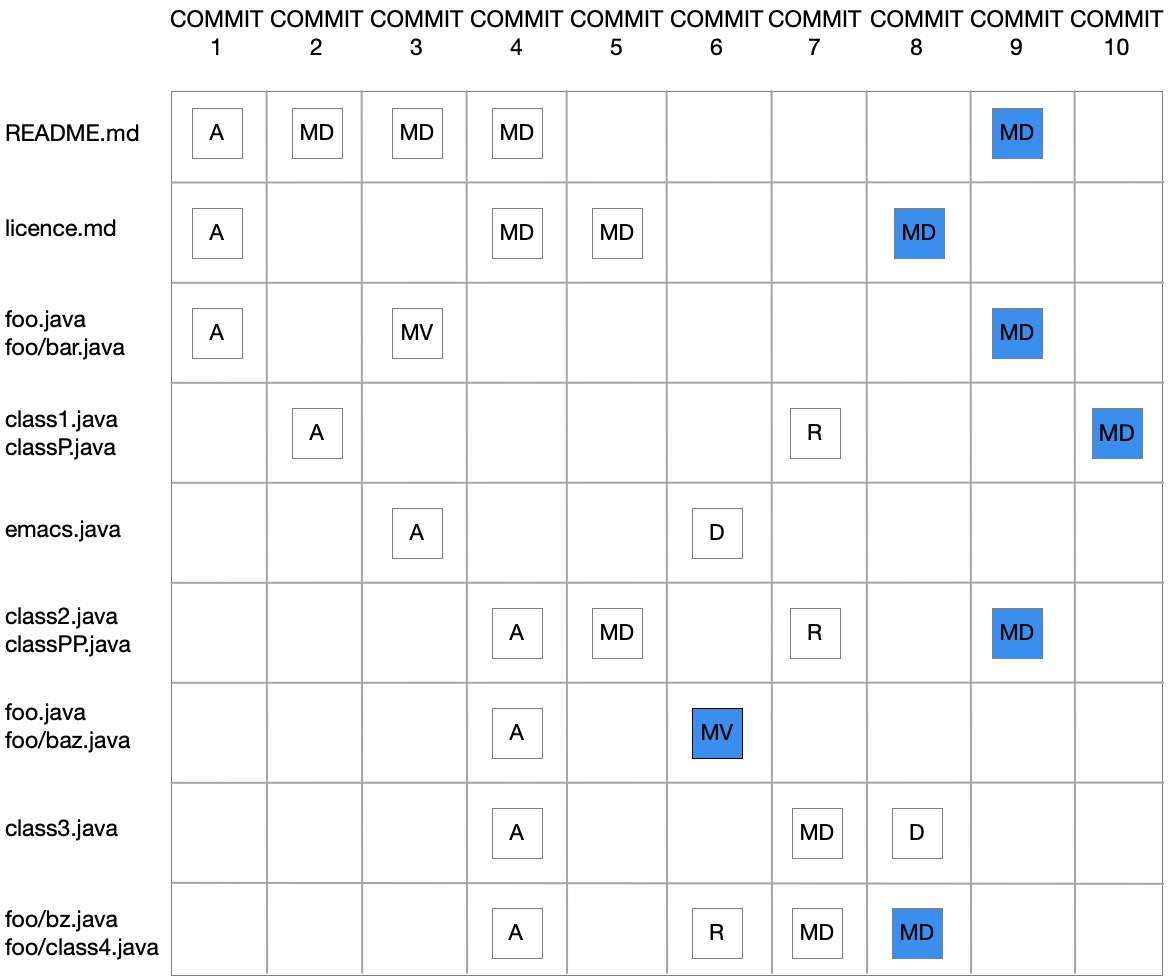
\includegraphics[width=0.6\textwidth]{2DMatrix.jpg}
    \caption{2D Representation of the structural evolution of a repository}
    \label{fig:evolutionMatrixApproach}
\end{figure}
\autoref{fig:evolutionMatrixApproach} depicts the evolution of a repository with 14 files and 10 commits. In this figure we only show the structural evolution of a repository, without considering file metrics as Lanza did. 
Each row represents the history of a file; therefore, it is associated with a set of FileVersions represented by the squares inside each cell. Actions on a file are labeled as: A for ADD, MD for MODIFY, MV for MOVE, R for RENAME, and D for DELETE.
As we can see, the first action made on each file is an ADD. Some files end their history with a DELETE. Notice that \texttt{foo.java} and \texttt{foo/bar.java} are represented by the same FileHistory because they represent the same logical entity in the system. 
In commit $C_3$, \texttt{foo.java} was moved under \texttt{foo/} and renamed to  \texttt{bar.java}.
The same goes for \texttt{foo.java} and \texttt{foo/baz.java} represented by the seventh FileHistory.

We can read this matrix as follows:
 \begin{itemize}
     \item \textbf{Vertically (by rows)}, if we are interested in the history of a particular entity. 
     For example, the FileHistory represented by the first row in \autoref{fig:evolutionMatrixApproach} represents the history of \texttt{README.md}, that was added in the first ProjectVersion (commit $C_1$) and then modified in the second, third, fourth, and ninth ProjectVersion.
     \autoref{fig:evolutionMatrixApproach} is an excellent example of why we cannot rely only on the file name to identify a system's entity. 
     We notice that \texttt{foo.java}, represented by the third FileHistory, was added with the first ProjectVersion and then moved with the third into \texttt{foo/bar.java}. 
     Then, in commit $C_4$, a new file \texttt{foo.java} was added. Nonetheless, the name of the files are the same, they represent two different entities. 
     \item \textbf{Horizontally (by columns)}, if we are interested in which entities were updated on each ProjectVersion. 
    For example, on the first ProjectVersion, we have added the \texttt{README.me} file, the \texttt{licence.md} file, and the \texttt{foo.java} file. 
 \end{itemize}

\autoref{fig:evolutionMatrixApproach} also provides an example of how we reconstruct the system's state after a commit. 
As we have seen, a ProjectVersion does not represent a system snapshot.
Instead, it represents only the changes made to the previous version. 
To reconstruct the system's state at a specific version, we need to consider, for each FileHistory, the last change before that version. 
Under those circumstances, for each FileHistory, we must go back in time until we find the rightmost change. Of course, if the rightmost difference was a DELETE, we ignore the related FileHistory.
In \autoref{fig:evolutionMatrixApproach}, the state of the system after $C_{10}$ is composed of the FileHistories that hold a row with a blue square. 



\subsection{3D Representation}
\label{s:3DRepr}
We aim to make an interactive 3D representation to ease the comprehension task of a developer. Interactive visualizations help users understand more information than a non-interactive version of the same graph. The interaction allows the user to discover a connection among the visualization elements. It is not easy to achieve the same result with a static visualization. For example, if we look at the graph of a repository activity on GitHub\footnote{\url{https://docs.github.com/en/repositories/viewing-activity-and-data-for-your-repository/analyzing-changes-to-a-repositorys-content\#visualizing-additions-and-deletion-to-content-in-a-repository}}, we cannot understand which file was modified at a given time. 

One advantage of our approach is the possibility of having multiple sources of information displayed simultaneously. We aim to make system analysis easier by using human senses and leveraging synesthesia. The phenomenon of synesthesia occurs when stimulation of a sense or a cognitive pathway leads to the involuntary stimulation of another reason or a cognitive path. We experience synesthesia when two or more events are perceived as the same. 
For example, synesthetic people might associate the red color with the letter D or the green color with the letter A. 
There are many forms of synesthesia, each representing different perceptions, such as visual forms, auditory, and tactile.

To visualize a project, we introduce the concept of \textbf{view}. We define a view as a way to illustrate the evolution of a project given a set of specifications. This set of specifications determines how the view must be built. For example, if we want to traverse the repository history by year, this information is part of the specification. A view holds a set of frames, called \textbf{AnimationFrame}, each representing the repository's state at a specific moment. Therefore, the entire history of the repository is displayed by rendering these AnimationFrames sequentially, like in a movie. 

Each repository has a unique history. There are young repositories whose history is one year long and old repositories with more than ten years of development activity. Many repositories are inactive on GitHub, whereas others might have a vast number of contributors raising the total number of commits daily. Therefore, we cannot provide a static approach to traverse the history of a repository. 
Every visualization has its own goal and its way of traversing time. For this reason, we provide two visualization strategies to group commits into AnimationFrames. Both of them traverse the whole history from the beginning until the end.
\begin{itemize}
    \item{Grouping by commits}: the user specifies the number of commits (\texttt{n}) and we create one AnimationFrame for every \texttt{n} commits. With this strategy, the concept of time is lost because we consider only the position of the commit in the commit tree.
    \item{Grouping by timestamp}: the user specifies a time window (\texttt{ts}) and we create one AnimationFrame for every \texttt{ts} seconds. All the commits inside the time window are part of the AnimationFrame. Therefore, we might have empty AnimationFrames if no commits are made in that time window.
\end{itemize}

\autoref{fig:TimeWindowExamples} shows an example of three strategies applied over the same history. In \autoref{fig:TimeWindow1} we made an AnimationFrame every 3 commits and as a result, the notion of time is lost. With a commit grouping strategy, we never have an empty AnimationFrame. In \autoref{fig:TimeWindow2} and \autoref{fig:TimeWindow3} the situation is different as they have empty AnimationFrames.
Overall, the examples highlight the importance of a well-designed time window and underline our need to leave the user the choice of the time window's length. For example, younger repositories might have a daily time window, while older repositories might have a weekly, monthly, or yearly view. 

\begin{figure}
    \begin{center}
        \begin{subfigure}{1\textwidth}
            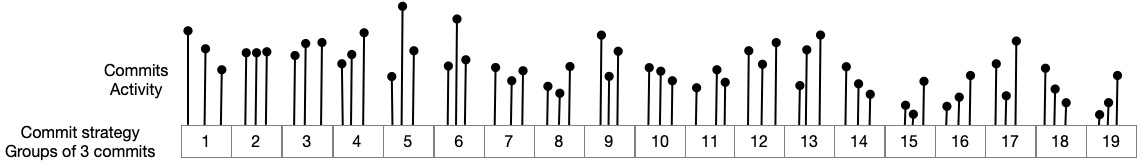
\includegraphics[width=\linewidth]{TimeWindow1.jpg}
            \caption{Grouping every 3 commits.} 
            \label{fig:TimeWindow1}
        \end{subfigure}
        \begin{subfigure}{1\textwidth}
            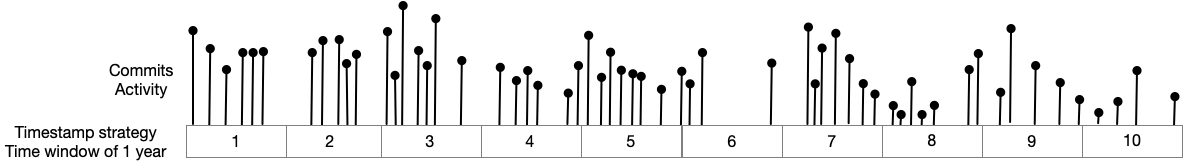
\includegraphics[width=\linewidth]{TimeWindow2.jpg}
            \caption{Grouping every year.} 
            \label{fig:TimeWindow2}
        \end{subfigure}
        \begin{subfigure}{1\textwidth}
            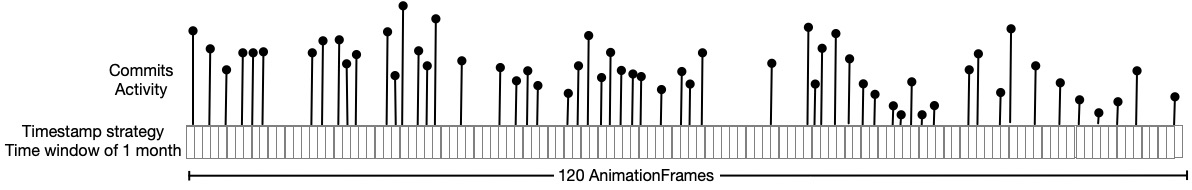
\includegraphics[width=\linewidth]{TimeWindow3.jpg}
            \caption{Grouping every month.}
            \label{fig:TimeWindow3}
        \end{subfigure}
        \caption[Example of three different grouping strategies]{Example of three different grouping strategies applied over a system whose history is 10 years long with 57 commits}
        \label{fig:TimeWindowExamples}
    \end{center}
\end{figure}



To represent the system's state, an AnimationFrame holds a set of \textbf{ViewFigures}, each representing a file of the system.

A ViewFigure holds a set of properties used by the render process to draw a glyph representing a file. 

\subsubsection*{Layout}
A layout specifies how graphical entities should be laid out. 
Various layout strategies have been proposed to visualize software evolution.
One of the most famous approaches is the city metaphor \cite{Wettel2007}, presented by Wettel \& Lanza, where a file's position depends on its package. It works very well with small and medium systems, and they stated that the interactivity and navigability could be substantially slowed down with large systems.

Our main goals are scalability and incrementality. The visualization needs to scale, even with a very large repository, and it must visualize the system's evolution incrementally. Therefore, the user can immediately distinguish older files from newer ones.

Under those circumstances, we adopted a spiral layout with an outward direction. It is shown in \autoref{fig:layout}. We set a constant gap between entities representing files. 
Older files are positioned at the center of this spiral, whereas newer files are always close to borders. 

We added the \textit{position} property to a ViewFigure to describe its location in the 3D environment. 

\begin{figure}
    \center
    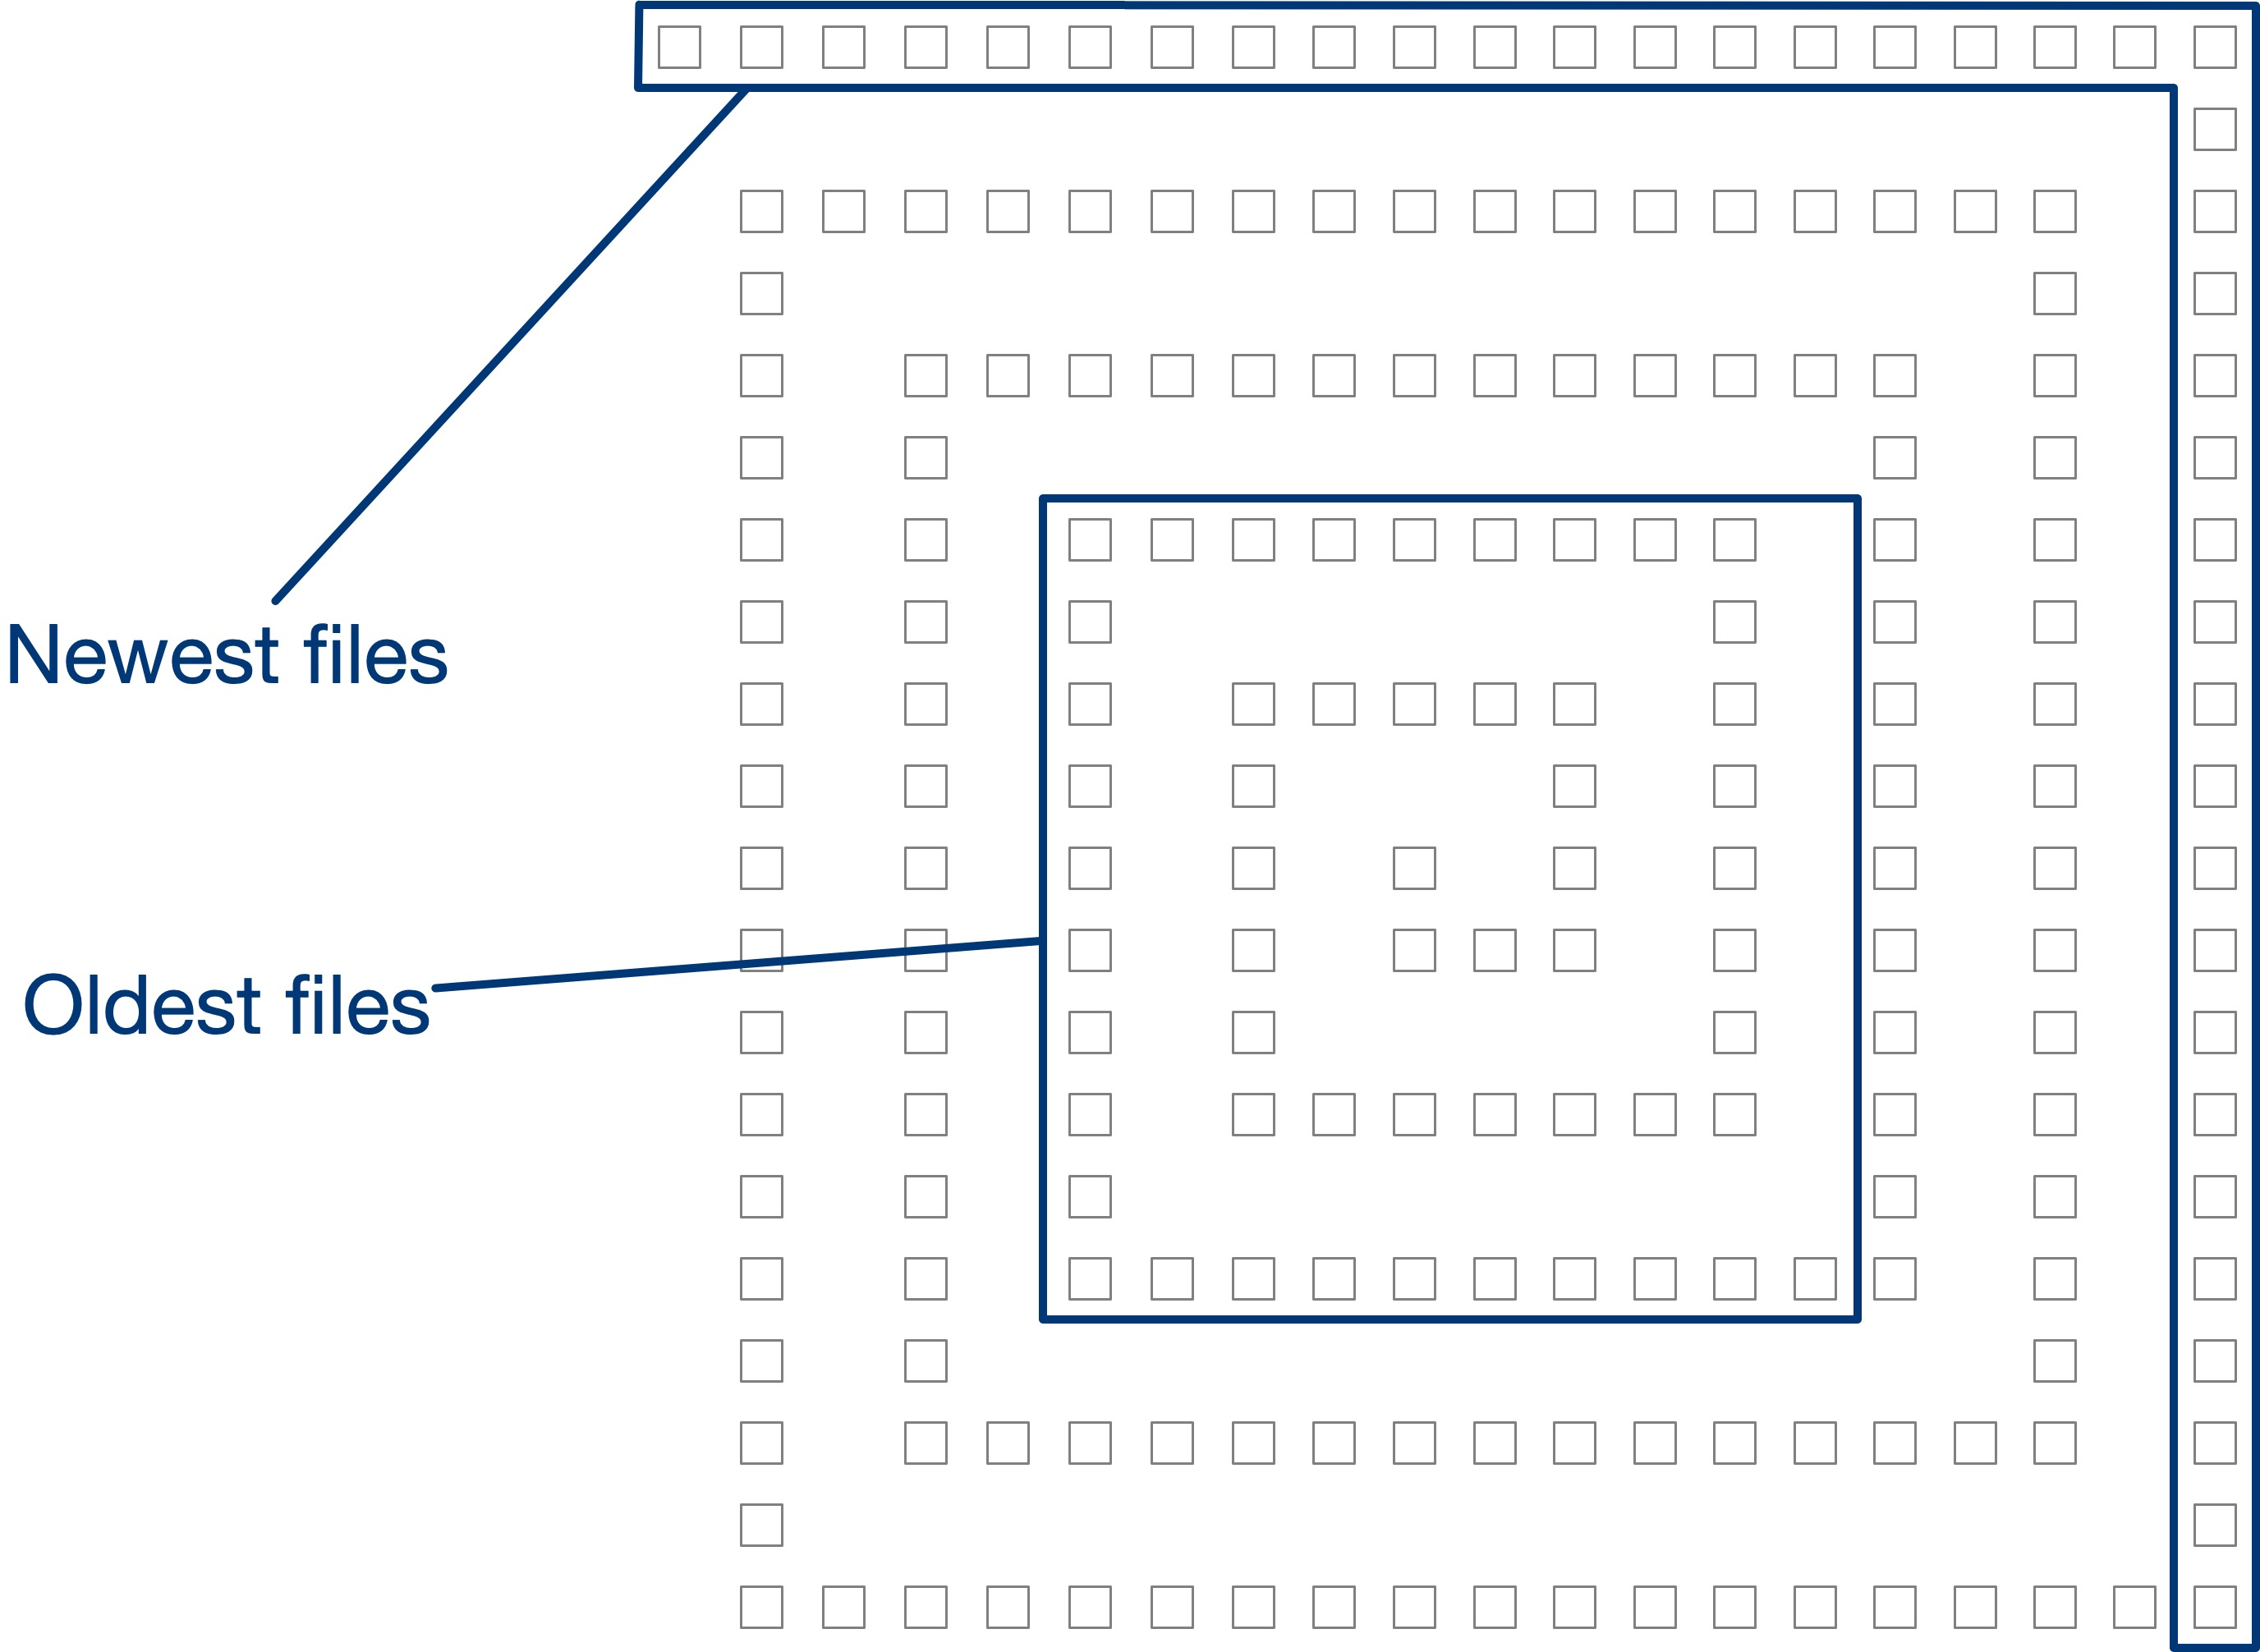
\includegraphics[width=0.7\textwidth]{SpiralLayout.jpg}
    \caption{Outward spiral layout}
    \label{fig:layout}
\end{figure}

\subsubsection*{Color}

Synesthesia occurs when we experience an involuntary stimulation of a cognitive path during the stimulation of another sense.
We present how we use color to describe file actions and simulate how time passes between actions.
As a result, we decided to map each git action with color (see \autoref{fig:ColorAssociation}). This mapping can be personalized through the \textit{color} property of ViewFigure.

In addition to the color, each ViewFigure has another property: \textit{age}. It represents the time elapsed between the last action made on a file and the currently displayed AnimationFrame. 
We selected two strategies to compute the age of an entity:

\begin{itemize}
    \item{Aging by commits}: the user specifies the number of commits (\texttt{n}), and then after \texttt{n} commits, the age of a file is incremented. 
    \item{Aging by timestamp}:  the user specifies a time window (\texttt{ts}) and then after \texttt{ts} seconds the age of a file is incremented.
\end{itemize}

When an action is made on a file, its age is reset to zero. 

The user also can set the maximum age.
When reached, the color of the entity must be equal to the \texttt{base color} chosen by the user.
 
We initially set the base color equal to grey.
\autoref{fig:Aging} provides an example of how the color of an entity changes toward the base color. In this figure, we used green as the base color and represented additions with ten aging steps. 


All the files shared the same criteria to compute the age. The primary purpose of the aging is to immediately distinguish files modified recently from files modified in past AnimationFrames.

\begin{figure}
    \center
    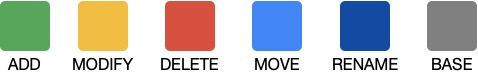
\includegraphics[width=0.5\textwidth]{ColorMapping.jpg}
    \caption{Mapped colors to git actions}
    \label{fig:ColorAssociation}
\end{figure}


\begin{figure}
    \center
    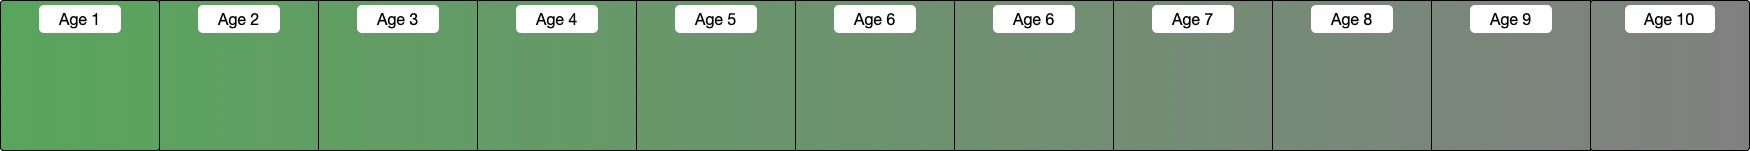
\includegraphics[width=\textwidth]{Aging.jpg}
    \caption{The aging process of an entity whose last action was an ADD and the maximum age is 10. }
    \label{fig:Aging}
\end{figure}



\subsubsection*{Shape and Opacity}
To easily distinguish file types, we added a \textit{shape} and an \textit{opacity} property to a ViewFigure.

We did not set a pre-defined set of shapes because we preferred to let each implementation have its own set of models. This was done because it is not guaranteed that all the visualization libraries share the same model. The idea is to map each file type with a shape previously selected by the user. 

Opacity was also added to allow the user to emphasize file types if needed. 


\subsubsection*{Height}
An important piece of information we want to represent is the value of a metric. SYN computes the values of a set of metrics, so we let the user choose his preference to map metrics to the files' height. \\


\autoref{fig:ApproachMapping} summarizes what we said so far. To visualize a Git repository, we use a view, a class that holds all the information needed to render it on screen. To depict the evolution, we traverse the repository's history by a group of commits (generated with a time window or every n commits). Each group is represented by an AnimationFrame, which holds a set of ViewFigures representing a file. The ViewFigure's position is used to describe the creation date of a file. The last action determines the color and age. A chosen metric is used to compute the height of the ViewFigure, and finally, the file type is mapped to shape and opacity. 


\begin{figure}
    \center
    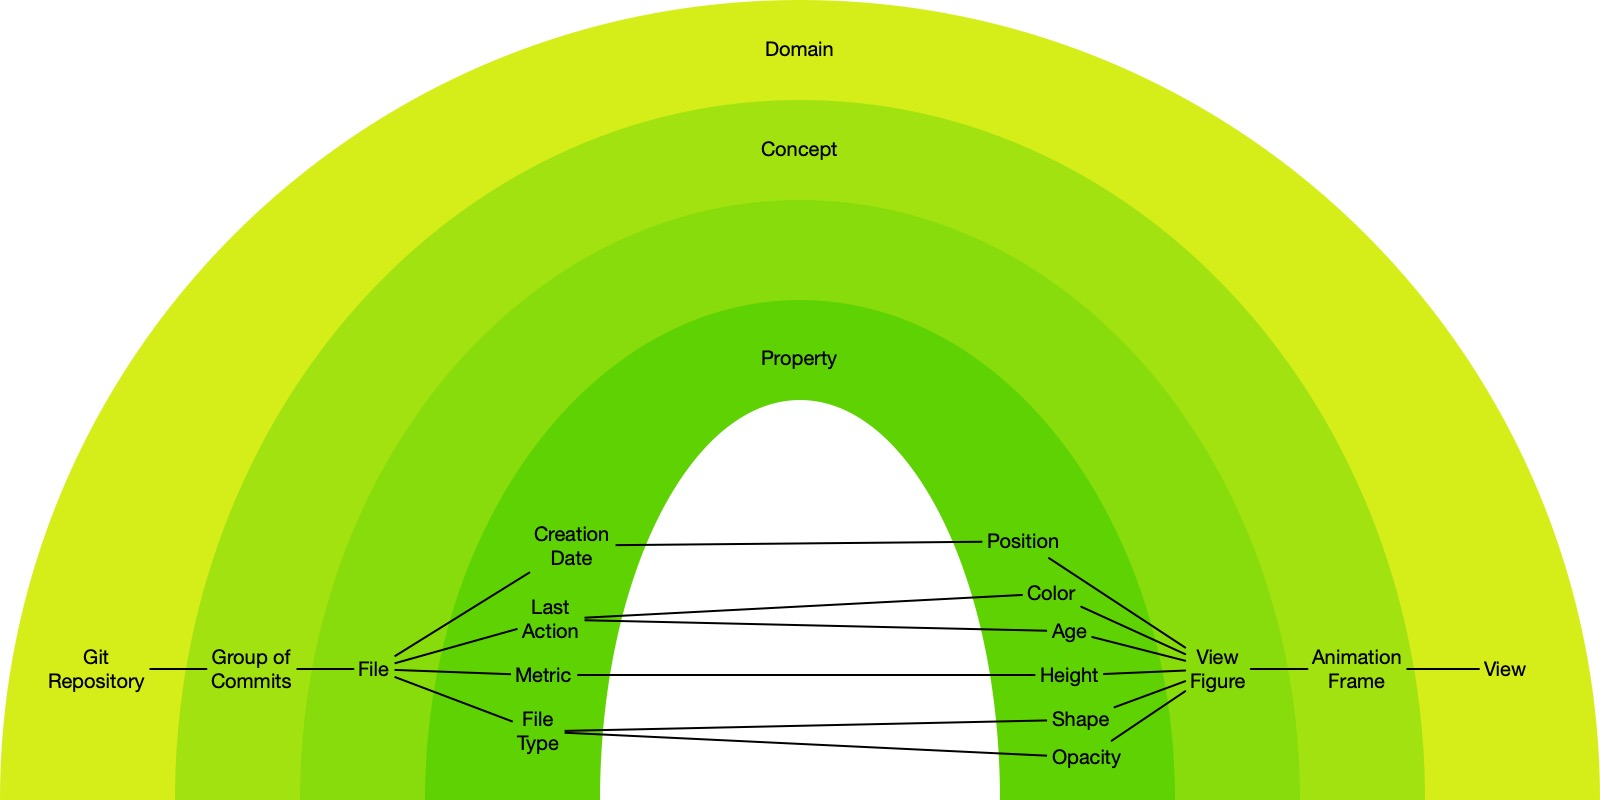
\includegraphics[width=\textwidth]{ApproachMapping.jpg}
    \caption{Mappings of file properties and metrics to view specifications}
    \label{fig:ApproachMapping}
\end{figure}


\newpage
\section{Evolution Auralization}
\label{sec:audioApproach}
In the previous sections, we detailed our approach to visualizing the evolution of a software system. In addition to sight, our approach also stimulates another sense: hearing. To complement our evolutionary visualization, we devised an approach to \emph{\quotes{auralize}} the evolution of a software system. Auralization is a term introduced to be used in analogy with visualization to describe rendering audible (imaginary) sound fields \cite{kleiner1993}. The intuition is to create a melody, starting from the evolutionary data extracted from the version control system, to augment our visualization with complementary pieces of information.


Many parameters influence a musical composition, such as beats per minute (i.e., BPM), pitch, or note. In our approach, we consider the following parameters:

\begin{itemize}
    \item \textbf{Tempo}: indicates the speed of a musical composition. It is measured in BPM. 
    \item \textbf{Measure}: represents a single unit of time featuring a specific number of beats. In our approach, this value is constant (i.e., 1 second). For every measure, we play a new AnimationFrame.
	\item \textbf{Pitch}: is the quality that makes it possible to judge sounds as \quotes{higher} and \quotes{lower} in a sense associated with musical melodies.
	\item \textbf{Amplitude}: determines how loud a note is (i.e., volume).
\end{itemize}

According to Vickerts \cite{Vickers2004}, to distinguish between different activities on the code, we need an \emph{\quotes{orchestral model}} where each instrument represents a certain activity. Following this idea, our approach is composed of three instruments, each representing a different aspect of the evolution of a software system:

\begin{itemize}

    \item \textbf{Bass drums} represents the \textbf{number of commits} in an AnimationFrame. We use this instrument also to dictate the \textbf{Tempo} of our musical composition: the higher the number of commits, the higher the tempo. We normalized the values in the interval $\left[60,200\right]$. The \textbf{amplitude} of this instrument is constant.
    
    \item \textbf{Bass sound} represents the number of \textbf{deleted files} in an AnimationFrame. We use the number of deleted files to determine the repetition and the amplitude of the sound. We divided the measure into quarters and play this instrument one to four times depending on the value of the metric represented. We linearly normalized the amplitude in the range $\left[0.1,0.8\right]$ depending on the metric's value.
    
    \item \textbf{Electric sound} represents the number of \textbf{added files} in an AnimationFrame. We use the number of deleted files to determine the repetition and the amplitude of the sound. We divided the measure into octaves and play this instrument one to eight times depending on the value of the metric represented. We linearly normalized the amplitude in the range $\left[0.2,0.85\right]$ depending on the metric's value.

\end{itemize}

The output of our approach is a musical composition representing a system's evolution. It should be noted that we obtained the parameters mentioned above by tuning the musical composition to our preference However, the approach is customized with different metrics or different thresholds. 


\begin{figure}
    \center
    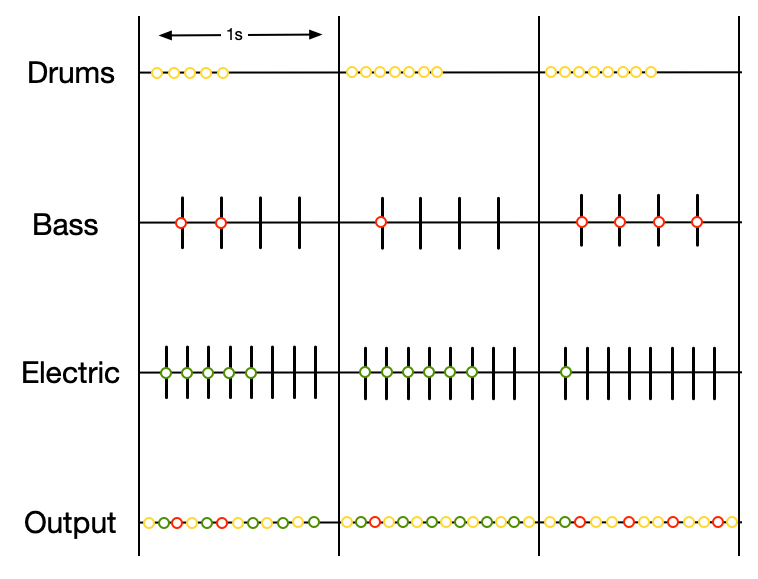
\includegraphics[width=0.5\textwidth]{AuralizationApproach.jpg}
    \caption{Example of how the auralization approach works. }
    \label{fig:ApproachArualization}
\end{figure}

\autoref{fig:ApproachArualization} provides an example of how this approach works. Each column represents a measure with a constant value of 1 second. Each row represents one instrument, except for the last, which represents the output composition. The number of notes played from each instrument depends on the value of the respective metric. Therefore, in all the measures was recorded an intense activity, especially in the third one. The number of deleted files was lower in the first two measures than in the last. Consequently, the final output is composed of a few bass notes on the first two measures and four bass notes on the last measure, the most active of this example. The same rules were applied for the electric sound, representing the number of added files.    
